\documentclass{article}
\usepackage[utf8]{inputenc}
\usepackage[spanish]{babel}
\usepackage{graphicx}
\usepackage{longtable}
\usepackage{float}
\usepackage{amsmath}
\usepackage{listings}
\graphicspath{{./img/}}
\usepackage{color}

\title{Práctica 4. Algoritmos Backtracking - Cena de Gala}

\author{Noelia Escalera Mejías \\
	\and Alejandro Menor Molinero \\
	\and Javier Núñez Suárez \\
	\and Adra Sánchez Ruiz \\
	\and Jesús Torres Sánchez}

\begin{document}
	\maketitle
	\section{Descripción del problema}
	Podemos describir el problema de la Cena de Gala de la siguiente forma:
	\\ 
	\\
	\textit{Se va a realizar una cela de gala a la que van a asistir n invitados. Cada invitado va a tener sentados junto a él a dos comensales (uno a su izquierda y otro a su derecha). Dependiendo de las características del invitado, existe una cierta conveniencia de que dos invitados se sienten juntos, definiendo la conveniencia global de la mesa como la suma de todos los niveles de conveniencia entre cada pareja de invitados sentados de forma contigua. El objetivo principal es conseguir sentar a los invitados de forma que el nivel de conveniencia global sea el máximo.}
	
	\
	
	Por tanto, nuestro algoritmo debe ser capaz de encontrar la asignación de invitados que maximice la afinidad de cada comensal con los otros dos comensales que tiene a su lado.
	\section{Representación del problema}
	La descripción del problema nos puede recordar mucho al problema del viajante de comercio.
	De hecho, se podría considerar el mismo problema con diferente enunciado.
	\
	
	Aquí en vez de ciudades, tenemos comensales. En vez de distancias, afinidades. En vez de minimizar, maximizar.
	
	\
	
	Para un número $n$ de comensales tenemos una tupla $(x_0, ..., x_{n-1})$ de ''sitios'' en la mesa. Siendo la afinidad global de la configuración: $\sum_{i=1}^{n-1} afinidad(x_i, x_{i-1}) + afinidad(x_i, x_{i+1})$, además de sumar la afinidad de $x_0$ y $x_{n-1}$ y viceversa.
	
	\section{Restricciones}
	Ya hemos visto como representar las decisiones que vamos haciendo (y deshaciendo) en el algoritmo. Es momento de hablar sobre que valores pueden tomar los elementos de la tupla.
	
	\
	
	\textbf{Restricciones explícitas}: Cada $x_i$ de la tupla que representa un estado del problema puede tomar un valor de $0$ a $n-1$ o $null$ si todavía no hemos llegado a esa decisión. Obviamente, en un estado solución no es posible este valor nulo, tenemos que sentar a todos los comensales en la mesa.

	\
	
	En cuanto a las \textbf{restricciones implícitas}: Una solución al problema tiene que ser una permutación de todos los comensales de $0$ a $n-1$, de forma que no podamos sentar al mismo comensal en dos sitios distintos de la mesa.
	
	\section{Descripción de las cotas usadas}
	En nuestra solución, hemos usado dos tipos de cotas: una \textbf{cota global}, que determina la máxima afinidad global encontrada hasta el momento. Si aún no se ha encontrado ninguna solución, estará inicializada de acuerdo a una versión Greedy del algoritmo. 
	
	\
	
	Por otro lado, también necesitamos una \textbf{cota local} (tal y como se ha mencionado anteriormente), necesaria para podar una rama en el caso de que la cota local (cota optimista) no supere a la cota global. La poda se puede realizar debido a que, si una cota local optimista genera peores resultados que una solución ya encontrada, esa rama no va a contener una solución mejor, por lo que no tiene sentido recorrerla.
	
	\
	
	Como detallaremos más adelante, para el cálculo de las afinidades optimistas de los comensales que quedan por seleccionar. Usaremos el promedio de sus dos mejores afinidades, como hemos visto de forma análoga en clase para el problema del viajante de comercio.
	
	\section{Representación de la solución}
	A la hora de representar el problema, hemos usado un TDA $Solucion$, para implementar nuestro algoritmo de \textit{backtracking} de una manera clara.
	\begin{itemize}
		\item \textbf{Información almacenada en el TDA $Solucion$}:
		\begin{itemize}
			\item \textit {x}: almacena la solución generada en cada momento. Se representa por medio de un vector de enteros (conceptualmente es un vector circular, representando la mesa para cenar), en el que cada componente toma el valor que representa el comensal que está sentado ahí.
			\item \textit{afinidades}: implementadas con una matriz, en la que cada elemento m[i][j] tiene asociado la conveniencia de sentar juntos al invitado i con el invitado j. Por tanto, deben coincidir m[i][j] con m[j][i].
			\item \textit {n}: es el número de comensales.
			\item \textit {solucionOptima}: almacena la mejor solución encontrada hasta el momento, es decir, la que tiene una mayor afinidad global.
			\item \textit {comensalesYaSentados}: es un vector de valores booleanos, su componente \textit{i} será \textit{true} si el comensal \textit{i} está ya sentado. Este vector nos permite comprobar la factibilidad en tiempo constante.
			\item \textit {afinidadActual}: contiene la afinidad acumulada para los comensales seleccionados en ese momento. Se usa para el cálculo de la afinidad de una solución obtenida y de la cota local de un nodo.
			\item \textit {Afinidades optimistas}: es un vector en el que su elemento \textit{i} es el promedio de sus dos mejores afinidades con otros dos comensales.
			\item \textit {AfinidadAcabarMesa}: Almacena la mejor afinidad del primer comensal seleccionado (que forzamos al comensal 0, para evitar soluciones equivalentes). La usamos para el cálculo de la cota local de un nodo.
		\end{itemize}
		\item \textbf{Operaciones del TDA Solucion}:
		\begin{itemize}
			\item \textit {Constructor}: realiza una serie de operaciones:
			\begin{itemize}
				\item Inicializa las variables del TDA a sus valores por defecto.
				\item Seleccionamos en primer lugar el comensal 0 para no generar soluciones equivalentes y reducir así el número de nodos hoja de $n!$ a $(n-1)!$.
				\item Inicializamos $solucionOptima$ y $maximoValor$ a partir de la versión Greedy (no óptima) del algoritmo.
				\item Calcula las $afinidadesOptimistas$ y la $afinidadAcabarMesa$ para evitar hacerlo posteriormente en el cálculo de las cotas locales. El proceso de estimación es bastante sencillo: para cada comensal, buscamos las dos mayores afinidades que tenga y le asociamos el promedio de ambas.
			\end{itemize}
			\item \textit {hemosTerminado(k)}: devuelve si ya hemos seleccionado el total de comensales ($k==n$).
			\item \textit {iniciaComp(k)}: inicializamos la componente k al valor NULO, que en nuestro caso es 0.
			\item \textit{sigValComp(k)}: asignamos a la componente k de la solución actual el siguiente valor ($x[k]++$).
			\item \textit{factible(k)}: para determinar su factibilidad, debemos comprobar si el comensal $x[k]$ ya estaba sentado en otro sitio, y si la afinidad acumulada hasta el momento y la estimación optimista de los comensales que quedan por seleccionar, es mayor que la cota global. 
			Si es factible, actualizamos la afinidad acumulada y el vector solución \textit{x}.
			\item \textit{todosGenerados(k)}: devuelve si se han generado todos los posibles comensales para $x[k], (x[k]==n)$. 
			\item \textit{procesaSolucion}: actualizamos la afinidad actual (sumándo la afinidad del último y el primero, para ''cerrar'' la mesa), la cota global y la solución óptima en el caso de que la afinidad actual sea mayor que la mejor solución obtenida.
			\item \textit{imprimeSolucion}: la utilizamos para comprobar que nuestro algoritmo funciona correctamente, imprime la mejor solución obtenida y su afinidad.
			\item \textit{vueltaAtras(k)}: deshace los cambios en la afinidadActual y en comensalesYaSentados (necesario para cuando damos una vuelta atrás en el algoritmo de Backtracking).
			\item \textit{cotaLocal(k)}: genera la cota local a partir de k. Para ello, obtiene la suma de las afinidadesOptimistas asociadas a los comensales que quedan por seleccionar.
		\end{itemize}
	\end{itemize}

	\section{Algoritmo Backtracking}
	El algoritmo sigue el esquema básico de los algoritmos Backtracking vistos en clase: 
	
	\begin{lstlisting}
	void backtracking(Solucion & sol, int k = 0){
		if (sol.hemosTerminado(k))
			sol.procesaSolucion();
		else{
			sol.iniciaComp(k);
			sol.sigValComp(k);
			while (!sol.todosGenerados(k)){
				if (sol.factible(k)){
					backtracking(sol, k+1);
					sol.vueltaAtras(k);
				}
				sol.sigValComp(k);
			}
		}
	}
	
	\end{lstlisting}
	
	
	
	\section{Estudio empírico}
	\begin{figure}[H]
		\centering
		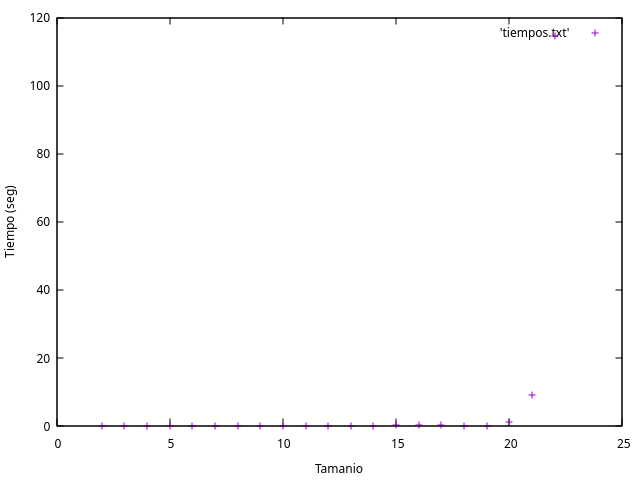
\includegraphics[totalheight=7cm]{grafica1}
		\caption{Tiempos de ejecución del algoritmo, desde tamaño 2 a 22}
		\label{fig:eficiencia_empirica}
	\end{figure}

	\begin{figure}[H]
		\centering
		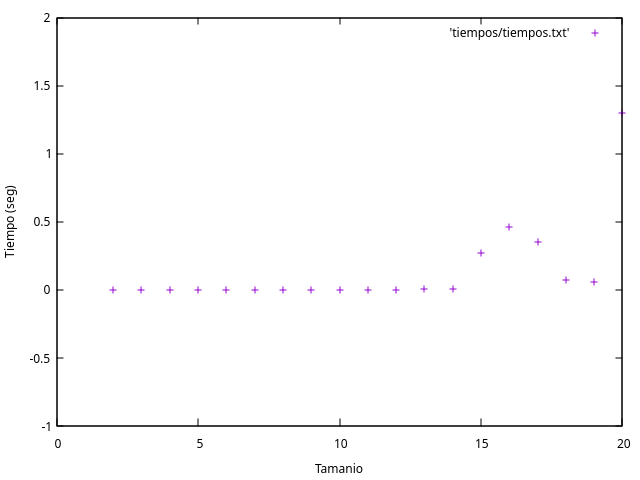
\includegraphics[totalheight=7cm]{grafica_intervalo_peque}
		\caption{Tiempos de ejecución del algoritmo con zoom en X en [0-20] y zoom en Y en [-1,2]}
		\label{fig:eficiencia_empirica_zoom}
	\end{figure}
	\section{Conclusiones}
	
\end{document}